\documentclass[10pt,a4paper]{article}
\usepackage[utf8]{inputenc}
\usepackage[portuguese]{babel}
\usepackage[T1]{fontenc}
\usepackage{amsmath}
\usepackage{mathtools}
\usepackage{amsfonts}
\usepackage{esint}
\usepackage{amssymb}
\usepackage{graphicx}
\usepackage[left=2.5cm,right=2.5cm,top=2.5cm,bottom=2.5cm]{geometry}
\usepackage{listings}
\usepackage{color} %red, green, blue, yellow, cyan, magenta, black, white
\definecolor{mygreen}{RGB}{28,172,0} % color values Red, Green, Blue
\definecolor{mylilas}{RGB}{170,55,241}

\newcommand{\prt}[1]{\left(#1\right)}
\newcommand{\col}[1]{\left[#1\right]}
\newcommand{\chv}[1]{\left\{#1\right\}}
\newcommand{\hgf}[4]{\prescript{}{2}{F}_1\left(#1,#2,#3,#4\right)}
\newcommand{\norm}[1]{\left\lVert#1\right\rVert}

\author{Murilo Camargos}
\title{Métodos Computacionais - Aula 7}
\begin{document}
\lstset{extendedchars=true, inputencoding=latin1,literate=
{á}{{\'a}}1
{à}{{\`a}}1
{ã}{{\~a}}1
{é}{{\'e}}1
{ê}{{\^e}}1
{í}{{\'i}}1
{ó}{{\'o}}1
{õ}{{\~o}}1
{ú}{{\'u}}1
{ü}{{\"u}}1
{ç}{{\c{c}}}1}
\lstset{language=Matlab,%
    %basicstyle=\color{red},
    breaklines=true,%
    morekeywords={matlab2tikz},
    keywordstyle=\color{blue},%
    morekeywords=[2]{1}, keywordstyle=[2]{\color{black}},
    identifierstyle=\color{black},%
    stringstyle=\color{mylilas},
    commentstyle=\color{mygreen},%
    showstringspaces=false,%without this there will be a symbol in the places where there is a space
    numbers=left,%
    numberstyle={\tiny \color{black}},% size of the numbers
    numbersep=9pt, % this defines how far the numbers are from the text
    emph=[1]{for,end,break},emphstyle=[1]\color{red}, %some words to emphasise
    %emph=[2]{word1,word2}, emphstyle=[2]{style},
    extendedchars=true,
    inputencoding=latin1, 
}

	\section{O problema de Sturm--Liouville}
	Seja o intervalo $I=[a,b]\subset\mathbb{R}$ e sejam $p$, $q$ e $r$ funções reais definidas em $I$, tais que:
	\begin{itemize}
		\item $p$ é contínua, diferenciável e estritamente positiva em $I$, ou seja, $p(x)>0$ para todo $x\in[a,b]$;
		\item $q$ é contínua em $I$;
		\item $r$ é contínua e estritamente positiva em $I$, ou seja, $r(x)>0$ para todo $x\in[a,b]$.
	\end{itemize}
	Para uma função $u$ definida em $I$ que seja pelo menos duas vezes diferenciável, vamos definir o operador diferencial $L$ por $(Lu)(x)=(p(x)u')'+q(x)u$. Entende-se por problema de Sturm--Liouville regular\footnote{Os trabalhos de Sturm e Liouville sobre o problema que é hoje conhecido como problema de Sturm--Liouville foram desenvolvidos entre 1829 e 1837.}, o problema de se determinar a função definida em $I$ e os números $\lambda$ tais que a seguinte equação diferencial seja satisfeita:
	\begin{equation}
		(Lu)(x) + \lambda r(x)u(x) = 0,
		\label{eq:1}
	\end{equation}
	com o seguinte tipo de condição de contorno: vamos supor que existam constantes reais $\alpha_1$, $\alpha_2$, $\beta_1$ e $\beta_2$ tais que $(\alpha_1,\alpha_2)\neq (0,0)$, $(\beta_1,\beta_2)\neq (0,0)$ e tais que o seguinte par de relação deve ser válido:
	\begin{equation}
		\alpha_1 u(a) + \alpha_2 u'(a) = 0, \hspace{0.5cm} \beta_1 u(b) + \beta_2 u'(b)=0.
	\end{equation}
	Se $\lambda$ for um número tal que a equação~\ref{eq:1} seja satisfeita para alguma função $u_\lambda$ (que, em geral, dependerá de $\lambda$) então diz-se que $\lambda$ é um autovalor do Problema de Sturm--Liouville e $u_\lambda$ é dito ser a autofunção associada ao autovalor $\lambda$ do Problema de Sturm--Liouville. Essa nomenclatura surge por analogia com os conceitos de autovalor e autovetor de matrizes na álgebra linear. Tal se justifica por, definindo-se o operador $M=-\frac{1}{r}L$, a equação $Lu_\lambda + \lambda ru_\lambda=0$, escreve-se na forma $Mu_\lambda=\lambda u_\lambda$, que é precisamente uma equação de autovalores para o operador $M$.
	\begin{itemize}
		\item \textbf{Produtos escalares}: Para o espaço linear real das funções contínuas definidas no intervalo $[a,b]$, podemos definir os produtos escalares reais por: \[(f,g) = \int_a^b f(x)g(x)\,dx \hspace{.3cm}\text{e}\hspace{.3cm}(f,g)_r = \int_a^bf(x)g(x)r(x)\,dx,\] em que a função $r$ é a função estritamente positiva caracterizada acima no problema de Sturm--Liouville.
		\item \textbf{Realidade dos autovalores}: Os autovalores de um Problema de Sturm--Liouville são números reais.
		\item \textbf{Realidade das autofunções}: As autofunções de um Problema de Sturm--Liouville podem ser escolhidas como funções reais.
		\item \textbf{Relação de ortogonalidade}: Sejam $u_{\lambda_1}$ e $u_{\lambda_2}$ duas autofunções reais associadas a dois autovalores distintos $\lambda_1$ e $\lambda_2$, então valo que: \[\int_a^b u_{\lambda_1}(x)u_{\lambda_2}(x)r(x)\,dx = 0.\] Esta solução é chamada função de ortogonalidade.
		\item \textbf{O quociente de Rayleigh}: Seja $u_\lambda$ uma autofunção (real) com autovalor $\lambda\in\mathbb{R}$, ou seja, tal que $(pu_\lambda')'+qu_\lambda+\lambda ru_\lambda = 0$. Multiplicando-se essa igualdade por $u_\lambda$ e integrando-se entre $a$ e $b$, tem-se:
		\begin{equation}
			\lambda\int_a^b u_\lambda^2(x)r(x)\,dx = -\int_a^bu_\lambda(x)(pu_\lambda')'(x)\,dx - \int_a^bu_\lambda^2(x)q(x)\,dx,
			\label{eq:3}
		\end{equation}
		vamos agora integrar por partes a primeira integral. Temos: \[\int_a^bu_\lambda(x)(pu_\lambda')'(x)\,dx = \left. (pu_\lambda u_\lambda')(x) \right|_a^b - \int_a^b(u_\lambda'(x))^2p(x)\,dx,\] substituindo em (\ref{eq:3}), tem-se: \[\lambda\int_a^b u_\lambda^2(x)r(x)\,dx = \int_a^b\left[(u_\lambda'(x))^2p(x)-u_\lambda^2(x)q(x)\right]\,dx + \left[p(a)u_\lambda(a)u_\lambda'(a)-p(b)u_\lambda(b)u_\lambda'(b)\right],\]
		o que permite escrever:
		\begin{equation}
			\lambda = \frac{\int_a^b\left[(u_\lambda'(x))^2p(x)-u_\lambda^2(x)q(x)\right]\,dx + \left[p(a)u_\lambda(a)u_\lambda'(a)-p(b)u_\lambda(b)u_\lambda'(b)\right]}{\int_a^b u_\lambda^2(x)r(x)\,dx}
			\label{eq:4}
		\end{equation}
		O lado direito de (\ref{eq:4}) é denominado quociente de Rayleigh e desempenha um papel importante na análise de propriedades dos autovalores de problemas de Sturm--Liouville regulares. O quociente de Rayleigh (\ref{eq:4}) é também usado para a determinação aproximada de autovalores a partir de aproximantes para as autofunções, de particular utilidade quando as soluções de problema de Sturm--Liouville não puderem ser obtidas de forma explícita. No exercício 1, da lista para amanhã, ilustramos em uma solução simples como esse cálculo aproximado de autovalores pode ser feito.
	\end{itemize}
	
	\section{Exercícios}
	Para cada caso da Tabela~\ref{tbl:1}, encontre os autovalores e autofunções associadas do Problema de Sturm--Liouville regular:
	\[u''(x)+\lambda u(x)=0, \hspace{.3cm} 0<x<L, \hspace{.3cm} \beta_1u'(0)+\alpha_1u(0)=0, \hspace{.3cm}\beta_2u'(L)+\alpha_2 u(L)=0\]
	
\begin{table}[!ht]
\centering
\label{tbl:1}
\begin{tabular}{lll}
 \hline
 & em $x=0$ & em $x=L$\\
 \hline
 1 & Dirichlet & Dirichlet\\
   & $\alpha_1\neq 0,\,\beta_1=0$ & $\alpha_2\neq 0,\,\beta_2=0$\\ 
 2 & Dirichlet & Neumann\\
   & $\alpha_1\neq 0,\,\beta_1=0$ & $\alpha_2=0,\,\beta_2\neq 0$\\ 
 3 & Dirichlet & Robin\\
   & $\alpha_1\neq 0,\,\beta_1=0$ & $\alpha_2\neq 0,\,\beta_2\neq0$\\ 
   
 4 & Neumann & Dirichlet\\
   & $\alpha_2=0,\,\beta_2\neq 0$ & $\alpha_2\neq 0,\,\beta_2=0$\\ 
 5 & Neumann & Neumann\\
   & $\alpha_2=0,\,\beta_2\neq 0$ & $\alpha_2=0,\,\beta_2\neq 0$\\ 
 6 & Neumann & Robin\\
   & $\alpha_2=0,\,\beta_2\neq 0$ & $\alpha_2\neq 0,\,\beta_2\neq0$\\
   
 7 & Robin & Dirichlet\\
   & $\alpha_2\neq 0,\,\beta_2\neq0$ & $\alpha_2\neq 0,\,\beta_2=0$\\ 
 8 & Robin & Neumann\\
   & $\alpha_2\neq 0,\,\beta_2\neq0$ & $\alpha_2=0,\,\beta_2\neq 0$\\ 
 9 & Robin & Robin\\
   & $\alpha_2\neq 0,\,\beta_2\neq0$ & $\alpha_2\neq 0,\,\beta_2\neq0$\\ 
 \hline
\end{tabular}
\caption{Condições de contorno}
\end{table}

Determine também, em cada caso, a norma quadrada:
\[\norm{u_\lambda}^2 = \int_0^L u_\lambda^2(x)\,dx\]

\newpage
\section{Resolução}
Primeiramente, vamos resolver o Problema de Sturm--Liouville regular. Podemos assumir que a solução do problema é exponencialmente proporcional a uma constante $\gamma$, de tal forma que $u = e^{\gamma x}$. Utilizando esta suposição no problema de segunda ordem, temos:
\begin{align*}
	u''(x)+\lambda u(x) &= \prt{e^{\gamma x}}'' + \lambda e^{\gamma x}\\
	&= \gamma^2 e^{\gamma x} + \lambda e^{\gamma x}\\
	&= \prt{\gamma^2+\lambda} e^{\gamma x}\\
	&= 0
\end{align*}
resolvendo isto para $\gamma$, temos que $\gamma = \pm i\sqrt{\lambda}$. A solução geral do problema pode ser escrita como uma combinação linear das soluções, da seguinte forma:
\begin{align*}
	u_\lambda(x) &= c_1e^{i\sqrt{\lambda}x} + c_2e^{-i\sqrt{\lambda}x}\\
	&= c_1\prt{\cos{\prt{\sqrt{\lambda}x}} + i\sin{\prt{\sqrt{\lambda}x}}} + c_2\prt{\cos{\prt{-\sqrt{\lambda}x}} + i\sin{\prt{-\sqrt{\lambda}x}}}\\
	&= (c_1+c_2)\cos{\prt{\sqrt{\lambda}x}} + i(c_2-c_1)\sin{\prt{\sqrt{\lambda}x}}\\
	&= k_1\cos{\prt{\sqrt{\lambda}x}} + k_2\sin{\prt{\sqrt{\lambda}x}}
\end{align*}
Podemos calcular as autofunções para cada caso da tabela inserindo as condições de contorno. Temos:
\begin{itemize}
	\item \textbf{Dirichlet, Dirichlet}. temos que $\alpha_1u(0)=0\rightarrow u(0)=k_1=0$, assim, podemos reescrever $u_\lambda(x)=k_2\sin{\prt{\sqrt{\lambda}x}}$, para $k_2$ dado e um autovalor $\lambda$ que satisfaça as duas condições de contorno ao mesmo tempo. Como sabemos que $k_1=0$ para atender à primeira, podemos calcular a segunda da seguinte maneira: \[k_2\sin{\prt{\sqrt{\lambda}L}} = 0,\]
vamos considerar o caso em que $k_2\neq 0$ para que estejamos olhando para uma solução não trivial. Assim, temos que $\sin{\prt{\sqrt{\lambda}L}} = 0$ e, portanto, \[\lambda = \prt{\frac{n\pi}{L}}^2, \hspace{1cm}n=1,2,3,\dots\]
	\[\norm{u_\lambda}^2 = k_2^2 \left(\frac{\pi }{2}-\frac{\sin \left(2 \pi  \sqrt{\lambda }\right)}{4 \sqrt{\lambda }}\right)\]
	
	\begin{figure}[h!]
    \centering
      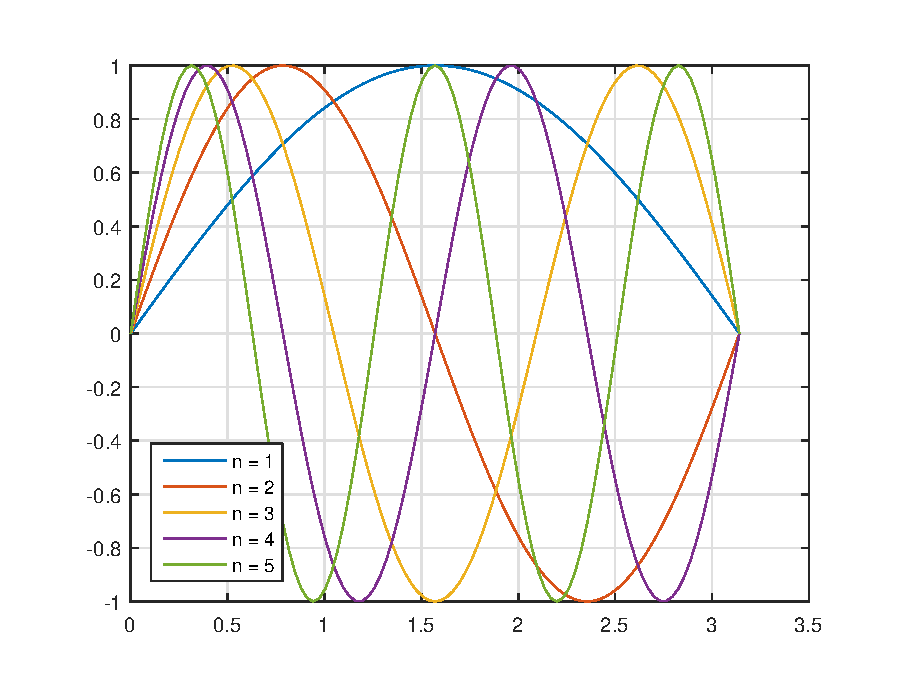
\includegraphics[scale=1]{figures/dd.eps}
	\end{figure}	
	
	\item \textbf{Dirichlet, Neumman}. temos que $\alpha_1u(0)=0\rightarrow u(0)=k_1=0$, assim, podemos reescrever $u_\lambda(x)=k_2\sin{\prt{\sqrt{\lambda}x}}$, para $k_2$ dado e um autovalor $\lambda$ que satisfaça as duas condições de contorno ao mesmo tempo. Como sabemos que $k_1=0$ para atender à primeira, podemos calcular a segunda da seguinte maneira: \[\sqrt{\lambda}k_2\cos{\prt{\sqrt{\lambda}L}} = 0,\]
vamos considerar o caso em que $k_2,\lambda\neq 0$ para que estejamos olhando para uma solução não trivial. Assim, temos que $\cos{\prt{\sqrt{\lambda}L}} = 0$ e, portanto, \[\lambda = \prt{\frac{(2n-1)\pi}{2L}}^2, \hspace{1cm}n=1,2,3,\dots\]

	\[\norm{u_\lambda}^2 = k_2^2 \left(\frac{\pi }{2}-\frac{\sin \left(2 \pi  \sqrt{\lambda }\right)}{4 \sqrt{\lambda }}\right)\]

	\begin{figure}[h!]
    \centering
      \includegraphics[scale=1]{figures/dn.eps}
	\end{figure}	

	\item \textbf{Neumman, Dirichlet}. de forma análoga aos exercícios anteriores, temos que
		\[u_\lambda(x)=k_1\cos{\prt{\sqrt{\lambda}x}}\]
		\[\lambda = \prt{\frac{(2n-1)\pi}{2L}}^2, \hspace{1cm}n=1,2,3,\dots\]
		\[\norm{u_\lambda}^2 =\frac{1}{4} k_2^2 \left(\frac{\sin \left(2 \pi  \sqrt{\lambda }\right)}{\sqrt{\lambda }}+2 \pi \right)\]
	\begin{figure}[h!]
    \centering
      \includegraphics[scale=1]{figures/nd.eps}
	\end{figure}	
	
	\item \textbf{Neumman, Neumman}
		\[u_\lambda(x)=k_1\cos{\prt{\sqrt{\lambda}x}}\]
		\[\lambda = \prt{\frac{n\pi}{L}}^2, \hspace{1cm}n=1,2,3,\dots\]
		\[\norm{u_\lambda}^2 =\frac{1}{4} k_2^2 \left(\frac{\sin \left(2 \pi  \sqrt{\lambda }\right)}{\sqrt{\lambda }}+2 \pi \right)\]
	\begin{figure}[h!]
    \centering
      \includegraphics[scale=1]{figures/nn.eps}
	\end{figure}	
\end{itemize}

\end{document}